\documentclass{jib}
\newlength{\platz}
\setlength{\platz}{15pt}
\RequirePackage{listings}

%\usepackage{changepage} %test, TODO remove

\lstset{%
  basicstyle=\ttfamily,
  fontadjust,
  flexiblecolumns=true,
  frame=L,
  xleftmargin=15pt,
  framesep=5pt,
  emphstyle=\rmfamily\itshape}
  

\usepackage{pdfpages}

%%%%%%%%%%%%%%%%%%%%%%%%%%%%%%%%%%%%%%%%%%%%%%%%%%%%%%%%%%
% JIB Header/Footer
%%%%%%%%%%%%%%%%%%%%%%%%%%%%%%%%%%%%%%%%%%%%%%%%%%%%%%%%%%
\jibvolume{XX} % insert volume
\jibissue{X}   % insert issue
\jibpages{XXX} % insert article ID
\jibyear{XXXX} % insert year
\makeHeaderFooter{} % leave as is
%%%%%%%%%%%%%%%%%%%%%%%%%%%%%%%%%%%%%%%%%%%%%%%%%%%%%%%%%%

\begin{document}

%%%%%%%%%%%%%%%%%%%%%%%%%%%%%%%%%%%%%%%%%%%%%%%%%%%%%%%%%%
%
% Title Page
%
%%%%%%%%%%%%%%%%%%%%%%%%%%%%%%%%%%%%%%%%%%%%%%%%%%%%%%%%%%

\begin{jibtitlepage}

\jibtitle{Synthetic Biology Open Language Visual (SBOL Visual) \\ Version 2.2}


%We did not provide author(s) nor author footnote(s), please complete as applicable.
% Please make sure to use unique footnote characters for each author
\jibauthor{
Hasan Baig\iref{uconn},
Pedro Fontanarossa\iref{utah},
Vishwesh Kulkarni\iref{warwick},
James McLaughlin\iref{newcastle},
Prashant Vaidyanathan\iref{msr},
Bryan Bartley\iref{bbn}, 
Swapnil Bhatia\iref{bu}, 
Shyam Bhakta\iref{rice},
Mike Bissell\iref{amyris},  
Kevin Clancy\iref{thermo}, 
Robert Sidney Cox\iref{kobe},
Angel Go\~{n}i Moreno\iref{newcastle},
Thomas Gorochowski\iref{bristol}, 
Raik Grunberg\iref{kaust},
Augustin Luna\iref{harvard}, 
Curtis Madsen\iref{bu},
Goksel Misirli\iref{keele},
Tramy Nguyen\iref{bbn}, 
Nicolas Le Novere\iref{babraham}, 
Zachary Palchick\iref{zymergen},
Matthew Pocock\iref{turing}, 
Nicholas Roehner\iref{bbn}, 
Herbert Sauro\iref{uw}, 
James Scott-Brown\iref{oxford},
John T. Sexton\iref{rice}, 
Guy-Bart Stan\iref{imperial}, 
Jeffrey J. Tabor\iref{rice}, 
Marta Vazquez Vilar\iref{upv},
Christopher A. Voigt\iref{mit}, 
Anil Wipat\iref{newcastle},
David Zong\iref{rice},
Zach Zundel\iref{utah}, 
Jacob Beal\iref{bbn},
Chris Myers\iref{utah}\jibauthorfootnote{*}{Correspondence should be addressed to:
           \email{editors@sbolstandard.org}}}

\addjibinstitution{uconn}{University of Connecticut, USA}
\addjibinstitution{utah}{University of Utah, USA}
\addjibinstitution{warwick}{University of Warwick, USA}
\addjibinstitution{newcastle}{Newcastle University, UK}
\addjibinstitution{msr}{Microsoft Research, UK}
\addjibinstitution{bbn}{Raytheon BBN Technologies, USA}
\addjibinstitution{bu}{Boston University, USA}
\addjibinstitution{rice}{Rice University, USA}
\addjibinstitution{amyris}{Shipyard Toolchains LLC, USA}
\addjibinstitution{thermo}{Thermo Fisher Scientific, USA}
\addjibinstitution{kobe}{Kobe University, Japan}
\addjibinstitution{bristol}{University of Bristol, UK}
\addjibinstitution{kaust}{KAUST, Saudi Arabia}
\addjibinstitution{harvard}{Harvard Medical School, USA}
\addjibinstitution{keele}{Keele University, UK}
\addjibinstitution{babraham}{Babraham Institute, UK}
\addjibinstitution{zymergen}{Zymergen, USA}
\addjibinstitution{turing}{Turing Ate My Hamster, Ltd., UK}
\addjibinstitution{uw}{University of Washington, USA}
\addjibinstitution{oxford}{University of Oxford, UK}
\addjibinstitution{imperial}{Imperial College, UK}
\addjibinstitution{upv}{Universitat Politecnica de Valencia, Spain}
\addjibinstitution{mit}{MIT, USA}


\end{jibtitlepage}


\begin{abstract}

People who are engineering biological organisms often find it useful to communicate in
diagrams, both about the structure of the nucleic acid sequences that they are engineering 
and about the functional relationships between sequence features and other molecular species.
%
Some typical practices and conventions have begun to emerge for such
diagrams.  The Synthetic Biology Open Language Visual (SBOL Visual) has been developed as a standard 
for organizing and systematizing such
conventions in order to produce a coherent language for expressing
the structure and function 
of genetic designs. 
%
This document details version 2.2 of SBOL Visual, which builds on the prior SBOL Visual 2.1 in several ways.
First, the grounding of molecular species glyphs is changed from BioPAX to SBO, aligning with the use of SBO terms for  interaction glyphs.
Second, new glyphs are added for proteins, introns, and polypeptide regions (e.g., protein domains),
the prior recommended macromolecule glyph is deprecated in favor of its alternative, and 
small polygons are introduced as alternative glyphs for simple chemicals.
\end{abstract}

This document does not contain technology or technical data controlled under either the U.S. International Traffic in Arms Regulations or the U.S. Export Administration Regulations.

\textbf{Keywords:} SBOL Visual; Standards; Diagrams

% Include your PDF document
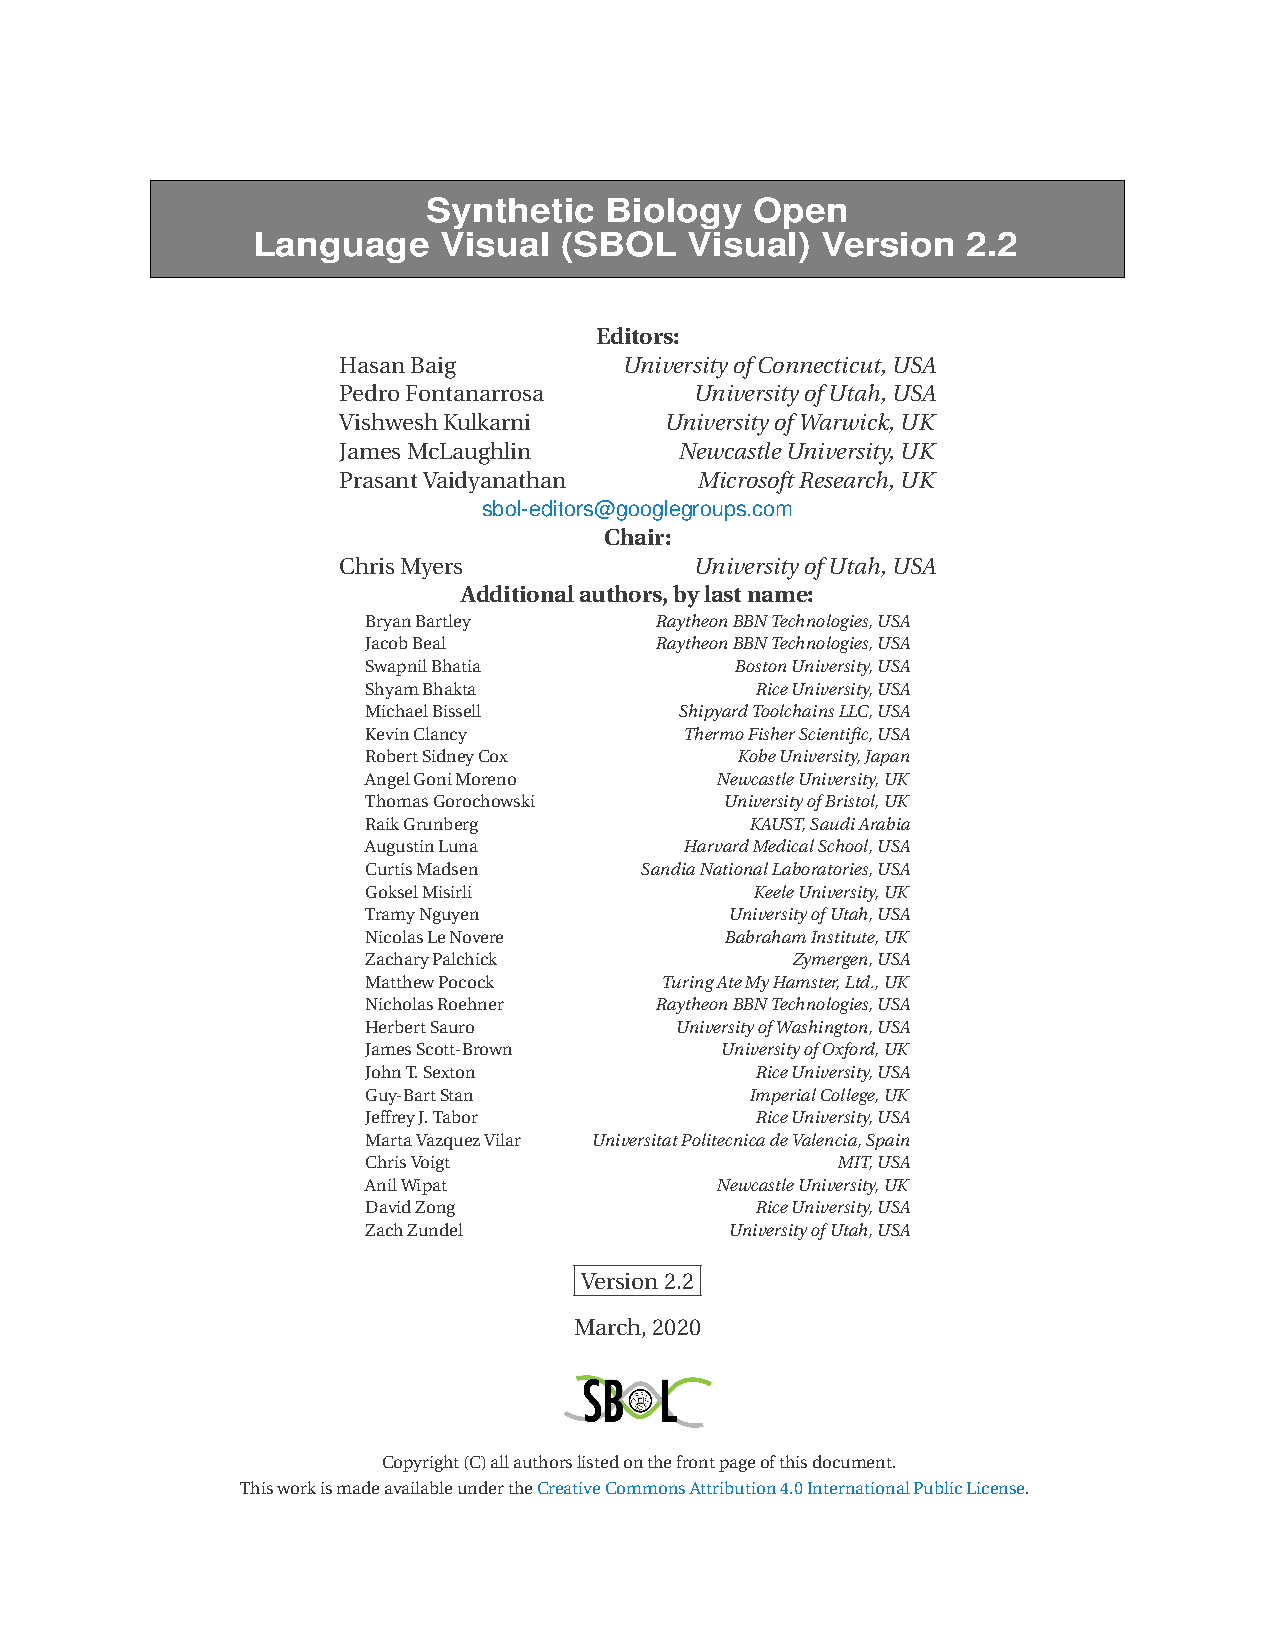
\includepdf[pages=-, offset=80 -80]{SBOL_Visual_2_2.pdf}

\end{document}
